\chapter*{Заключение}
\addcontentsline{toc}{chapter}{Заключение}

В результате выполнения лабораторной работы были изучены принципы функционирования, построения и особенности архитектуры суперскалярных конвейерных микропроцессоров.

Также были рассмотрены принципы проектирования и верификации сложных цифровых устройств с использованием языка описания аппаратуры SystemVerilog и ПЛИС.

На основе изученных материалов был найден способ оптимизации программы.

Поставленная цель достигнута.

\chapter*{Приложение}
\addcontentsline{toc}{chapter}{Приложение}

\begin{figure}[h]
	\centering
	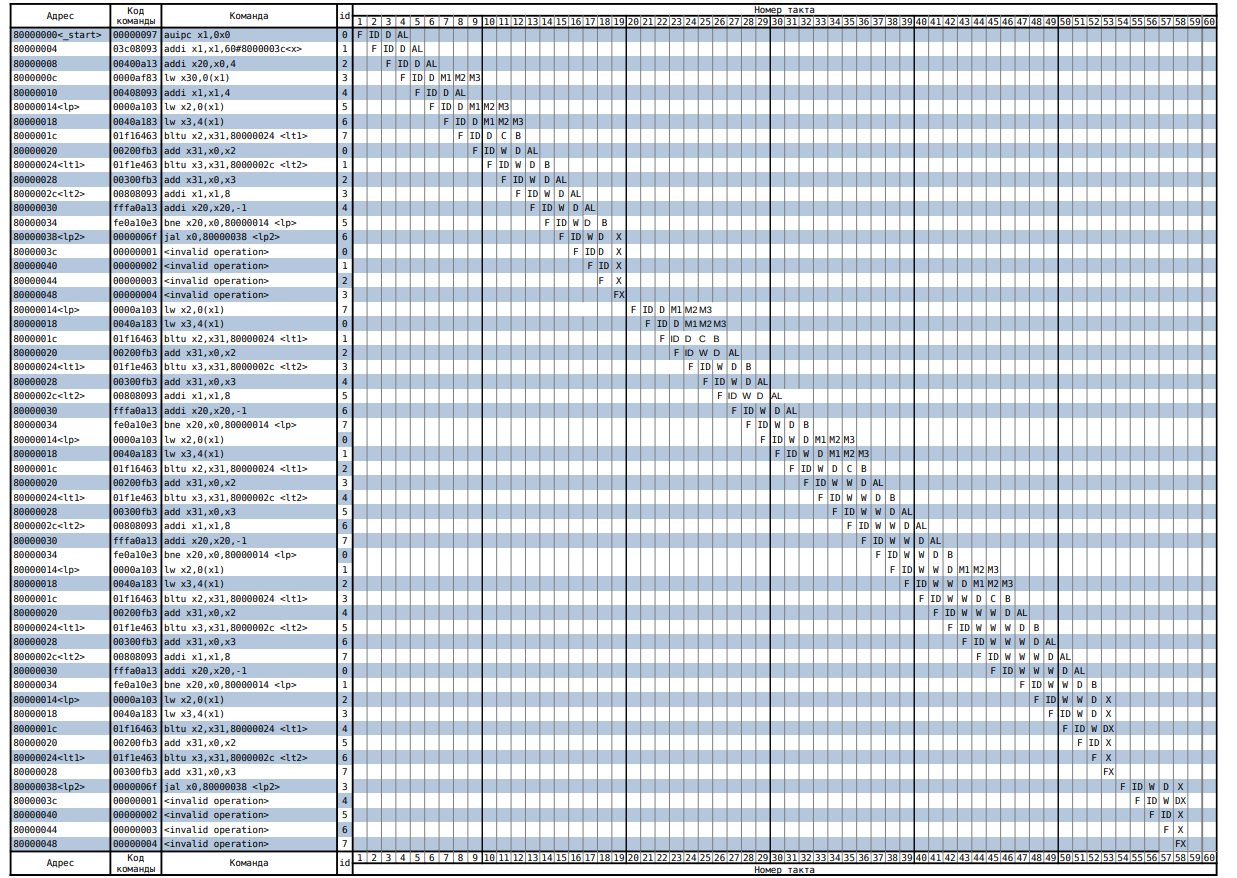
\includegraphics[height=0.33\textheight]{img/pipeline}
	\caption{Трасса работы программы.}
\end{figure}

\begin{figure}[h]
	\centering
	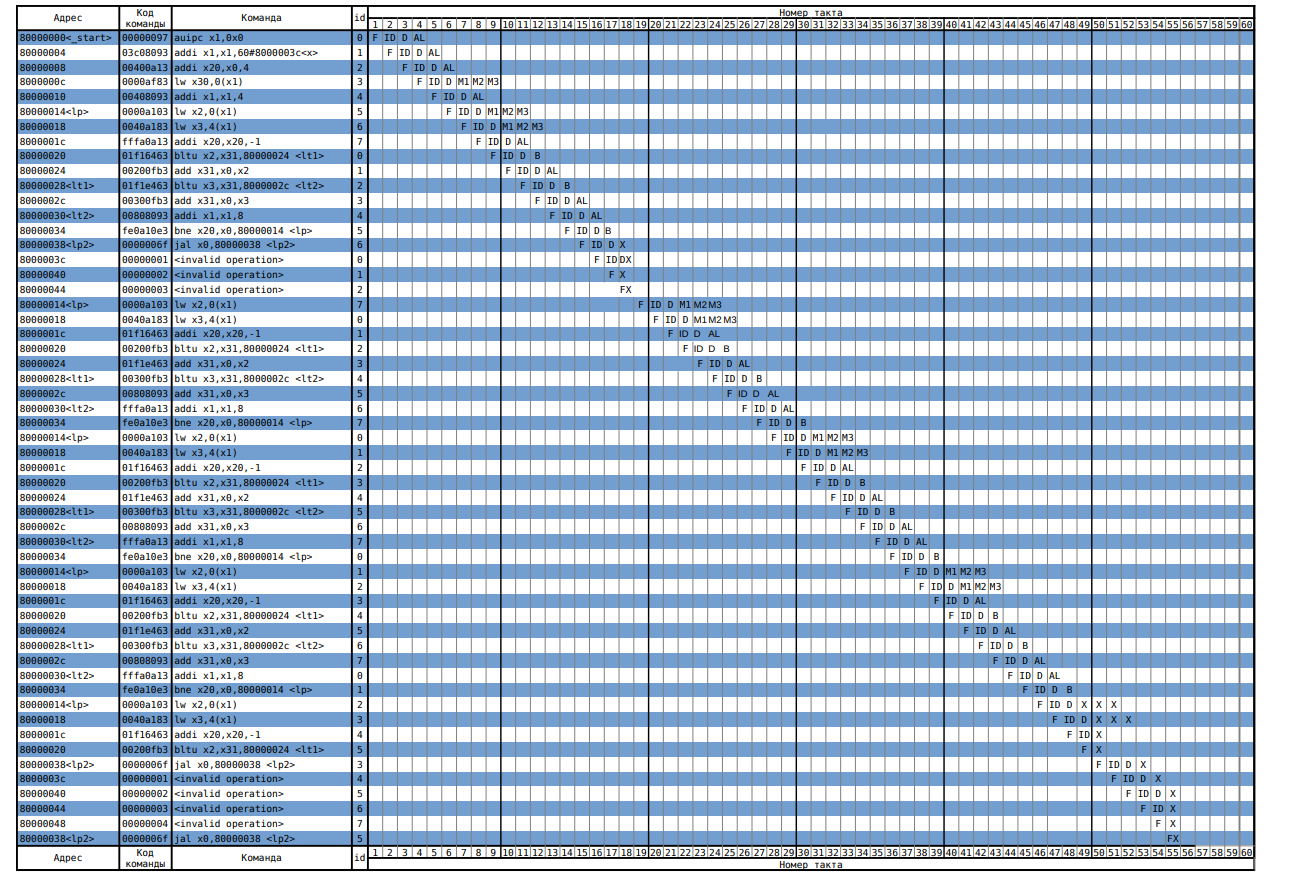
\includegraphics[height=0.33\textheight]{img/pipeline_op}
	\caption{Трасса работы оптимизированной программы.}
\end{figure}

